\documentclass[runningheads]{llncs}
\usepackage[T1]{fontenc}
\usepackage{graphicx}
\usepackage{amsmath}
\usepackage{booktabs}
\usepackage{array}
\usepackage{url}
\usepackage{float}
\usepackage[section]{placeins}
\newcommand{\method}{GRAIN-CAN}
\newcommand{\fpr}{\mathrm{FPR}}
\newcommand{\fnr}{\mathrm{FNR}}
\newcommand{\tpr}{\mathrm{TPR}}
\emergencystretch=2em
\begin{document}
\raggedbottom

\title{\method{}: Same-ID Local Behavior Residuals for Cross-Shift CAN Intrusion Detection}
\titlerunning{\method{}}
\author{Qi'ao Li}
\authorrunning{Q. Li}
\institute{School of Cyber Science and Technology, Beihang University, Beijing, China\\
\email{qi\_aolee@buaa.edu.cn}}
\maketitle

\begin{abstract}
Cross-vehicle CAN intrusion detection is difficult because both vehicle-specific message distributions and attack patterns can shift between training and deployment. Raw fixed-window representations add another difficulty: a short injection or spoofing burst may occupy only a few frames inside a long mostly normal window. This paper proposes \method{}, a supervised feature-based CAN IDS pipeline that exposes same-ID local behavior residuals before window aggregation. For each CAN frame, \method{} maintains a per-ID history state and extracts timing residuals, payload-change residuals, payload statistics, and local ID-behavior features using only current and past traffic. These frame-level features are aggregated with a fixed pre-test window configuration and classified by a lightweight supervised detector. We evaluate \method{} on CT\&T Test01--Test04 using attack-positive precision, recall, F1, FNR, FPR, and confusion matrices, with AUPR and fixed-FPR recall reported only as supplementary score-based evidence. The results show that same-ID residual features improve over raw fixed-window baselines in the hardest shifted settings, while ablation identifies timing residuals as the dominant signal in the current implementation.
\keywords{CAN bus \and Intrusion detection \and Automotive security \and Feature pipeline \and Cross-vehicle detection}
\end{abstract}

\section{Introduction}
Modern vehicles rely on controller area network (CAN) buses for communication among electronic control units. CAN is compact and efficient, but it does not authenticate message origin or payload integrity. Practical vehicle-security studies have shown that these properties leave room for malicious message injection and remote attack paths~\cite{koscher2010,checkoway2011,miller2015}. CAN intrusion detection systems therefore infer abnormal behavior from fields available on the bus: timestamps, arbitration IDs, data length codes, and payload bytes.

A closed-split detector can learn strong regularities from one vehicle and one attack family, but cross-shift detection is harder. A detector trained on one vehicle may encounter different CAN-ID frequencies, timing profiles, and payload ranges on another vehicle. Unknown-attack evaluation adds a second shift because the attack family and script may also change. In this setting, a detector that mainly memorizes absolute IDs, raw payload values, or a particular attack script can fail under deployment-like shifts.

Raw fixed-window representations create a second failure mode. CAN attacks are often local in both time and ID space: a short burst may affect a few frames while the rest of the window remains normal. If the model receives only a raw sequence or a coarse window summary, the abnormal frames can be diluted before classification. This does not mean raw sequence models are weak in general; as our results show, a raw Transformer can perform well in the known setting. The problem is stability under vehicle and attack shifts.

\method{} is built around one design insight: before forming a window, convert each frame into local behavior residuals relative to recent history of the same CAN ID. The pipeline maintains a per-ID state, extracts timing residuals, payload-change residuals, payload statistics, and local ID-behavior features, aggregates these frame-level signals using a fixed pre-test window, and trains a supervised detector. The final classifier is intentionally lightweight; the representation before aggregation is the contribution.

The paper makes two contributions.
\begin{enumerate}
  \item We propose \method{}, a supervised feature-based CAN IDS pipeline that exposes same-ID local behavior residuals before fixed-window aggregation. The pipeline makes short local attack evidence visible before it is diluted by long raw windows and reduces reliance on vehicle-specific absolute CAN distributions.
  \item We provide a controlled CT\&T cross-shift evaluation using attack-positive precision, recall, F1, FNR, FPR, confusion matrices, raw-window comparisons, window sensitivity, and feature ablation. The experiments separate representation effects from window choice and treat score-based metrics only as supplementary operating evidence.
\end{enumerate}

\section{Background and Design Motivation}
\subsection{CAN IDS Under Vehicle and Attack Shifts}
CAN IDS methods have used timing intervals, ID frequency, payload evolution, transition structure, physical-layer fingerprints, learned sequence representations, signal-level reconstruction, and graph-style representations~\cite{song2016,taylor2015,cho2016,cho2017,shahriar2022,wang2023}. Datasets such as ROAD and CT\&T make benchmarked CAN IDS evaluation more concrete~\cite{verma2020,blevins2021,lampe2024}. CT\&T is especially useful here because its settings separate known-vehicle/known-attack, unknown-vehicle/known-attack, known-vehicle/unknown-attack, and unknown-vehicle/unknown-attack cases.

\subsection{Why Raw Fixed Windows Can Lose Local Evidence}
Consider a window of $W$ frames. If only $k \ll W$ frames carry an injection artifact, a raw sequence model must both detect the local event and keep it visible after internal pooling, attention, or classification. The burden increases when the test vehicle changes, because the model must distinguish attack-induced perturbations from benign shifts in ID frequencies or payload ranges. \method{} addresses this by computing local residuals at the frame level, before the window is formed.

\subsection{Design Insight: Same-ID Local Residuals}
CAN IDs often exhibit repeated behavior. Rather than representing a frame only by absolute payload bytes or a raw position inside a window, \method{} asks how the current frame differs from recent frames with the same ID. This produces residual evidence: a timing gap, a payload-change magnitude, payload summary shifts, and local concentration changes. These residuals are not vehicle-independent, but they reduce dependence on absolute values of one vehicle and expose local disruptions that may recur across injection, spoofing, replay, flooding, and masquerade attacks.

\begin{figure}[t]
\centering

\includegraphics[width=0.98\textwidth]{figures/fig1_pipeline.pdf}
\caption{\method{} detector pipeline. The method maintains per-ID history, computes same-ID local residual features, aggregates them with a pre-test window configuration, and applies a lightweight supervised detector. Evaluation metrics are outside the pipeline.}
\label{fig:pipeline}
\end{figure}

\begin{figure}[t]
\centering

\includegraphics[width=0.92\textwidth]{figures/fig2_mechanism.pdf}
\caption{Feature-before-window mechanism. Sparse abnormal frames can be hidden inside a raw long window, while same-ID residual extraction turns the same local event into visible timing or payload-change spikes before aggregation.}
\label{fig:mechanism}
\end{figure}

\section{\method{} Pipeline}
\subsection{Overview}
\method{} is a detector pipeline, not a neural architecture. It consists of four stages: per-ID history maintenance, frame-level local residual extraction, fixed pre-test window aggregation, and supervised classification. Unlike raw-window neural detectors that learn directly from a fixed sequence of frames, \method{} first converts each frame into local behavior residuals with respect to the recent history of the same CAN ID.

\subsection{Input Stream and Per-ID History State}
The input stream is an ordered sequence $x_i=(t_i,id_i,dlc_i,b_i)$, where $t_i$ is the timestamp, $id_i$ is the arbitration ID, $dlc_i$ is the data length, and $b_i$ denotes the payload bytes padded or masked to a fixed byte representation. For each CAN ID, \method{} maintains a compact state
\[
H_{id}=\{t^{last}_{id}, b^{last}_{id}, c^{local}_{id}, s^{local}_{id}\},
\]
where $t^{last}_{id}$ and $b^{last}_{id}$ are the most recent timestamp and payload of that ID, $c^{local}_{id}$ stores recent occurrence counts, and $s^{local}_{id}$ stores summary statistics needed by implemented features. The state is updated online. During test-time inference, it uses only current and past frames.

\subsection{Same-ID Local Behavior Features}
For a frame $x_i$, \method{} computes feature groups with different purposes.

\paragraph{Timing residuals.} The same-ID time gap is
\[
\Delta t_i = t_i - t^{last}_{id_i}.
\]
where $t^{last}_{id_i}$ is the previous timestamp of the same CAN ID. This feature exposes injection, flooding, replay, or scheduling disruptions that change inter-arrival behavior.

\paragraph{Payload-change residuals.} Let $b_i$ be the current payload vector and $b^{last}_{id_i}$ the previous payload of the same ID. A simple implemented residual is
\[
\Delta b_i^{(1)} = \lVert b_i-b^{last}_{id_i}\rVert_1.
\]
where the norm is computed over available payload bytes. This group captures byte-level discontinuity without requiring signal decoding.

\paragraph{Payload statistics.} The pipeline also records coarse byte summaries such as sum, mean, standard deviation, and extrema. These features are weaker than decoded physical signals, but they are available when DBC files or signal definitions are absent.

\paragraph{Local ID behavior.} Local ID features summarize short-window concentration, frequency, and related count statistics. They are intended to capture abnormal bursts or shifts in local ID composition.

The current ablation shows that same-ID timing residuals dominate the CT\&T Test04 setup. Payload and ID features remain part of the modular representation, but they should not be overstated as the primary source of gain in the present results.

\subsection{Window Construction and Labeling}
Frame-level features are aggregated into fixed windows such as W10, W20, or W100. The window size is fixed before final test evaluation, or selected only on a validation split if such a procedure is explicitly available. In the current evidence package, W10/W20/W100 are reported as sensitivity configurations rather than test-selected winners. A window is labelled attack if any frame in the window is labelled attack. This label rule is common in window-level IDS experiments, but it also creates normal-dominated attack windows; \method{} is designed to keep local residuals visible before this window label is applied.

\subsection{Supervised Detector and Score Output}
In the repository experiments, \method{} is instantiated with a gradient-boosting tree ensemble. The classifier is not the contribution by itself; it learns a joint decision boundary over interpretable same-ID residual features. When the classifier exposes a score, AUPR and fixed-FPR recall are reported as supplementary operating evidence. The main decision metrics remain thresholded precision, recall, F1, FNR, FPR, and confusion-matrix counts.

\begin{table}[t]
\caption{Pipeline components and leakage controls.}
\label{tab:components}
\centering\small
\setlength{\tabcolsep}{3pt}
\begin{tabular}{p{0.21\textwidth}p{0.22\textwidth}p{0.23\textwidth}p{0.25\textwidth}}
\toprule
Component & Input & Output & Purpose / control \\
\midrule
Per-ID state & Ordered CAN frames & Last time, last payload, local counters & Online history; no future frames \\
Local residual extractor & Current frame + same-ID state & Timing, payload, ID-behavior features & Expose local changes before aggregation \\
Fixed window aggregation & Frame-level residuals & Window feature vector & Produce supervised samples; W fixed before test \\
Supervised detector & Window features + training labels & Score and label & Learn joint boundary; threshold not test-tuned \\
\bottomrule
\end{tabular}
\end{table}

\subsection{Training and Inference Protocol}
\begin{table}[t]
\caption{Algorithmic view of \method{} training and inference.}
\label{tab:algorithm}
\centering\small
\begin{tabular}{p{0.47\textwidth}p{0.47\textwidth}}
\toprule
Training phase & Inference phase \\
\midrule
Fix feature definitions and candidate window configuration. & Freeze feature definitions, window size, detector, and threshold. \\
Process training frames in timestamp order and update per-ID histories. & Process the test stream once in timestamp order. \\
Compute same-ID timing, payload-change, payload-statistical, and ID-behavior features. & Compute features from current and previous frames only. \\
Aggregate frame-level features into fixed windows and assign window labels. & Aggregate with the fixed window configuration. \\
Fit the supervised detector using normal/attack labels. & Emit score or label before using test labels for evaluation. \\
Select threshold on validation data when a score threshold is required. & Do not tune threshold, features, or window length on the test split. \\
\bottomrule
\end{tabular}
\end{table}

\subsection{Relation to Existing Pipeline Types}
\method{} is narrower than signal-level, graph, and self-supervised frameworks. It does not require DBC files, decoded physical signals, or a deep backbone. It also does not claim arbitrary zero-day detection, because it is supervised. Its role is to test whether a lightweight residual representation before aggregation improves cross-shift supervised CAN IDS.

\begin{table}[t]
\caption{Positioning against representative CAN IDS pipeline families.}
\label{tab:positioning}
\centering\small
\setlength{\tabcolsep}{3pt}
\begin{tabular}{p{0.15\textwidth}p{0.30\textwidth}p{0.22\textwidth}p{0.23\textwidth}}
\toprule
Work & Core mechanism & Required information & Relation to \method{} \\
\midrule
CANShield~\cite{shahriar2022} & Signal-level multi-scale autoencoder framework & Signal extraction / DBC-like information & Stronger signal semantics; heavier information requirement \\
X-CANIDS~\cite{xcanids2023} & Signal-aware explainable detection & CAN database / signal semantics & More explainable when signals are known \\
CANet~\cite{canet2019} & Unsupervised neural detection & Raw CAN messages & Benign-only training; different supervision assumption \\
StatGraph~\cite{wang2023} & Multi-view statistical graph learning & Message graph construction & Models relationships; heavier representation \\
\method{} & Same-ID residuals before aggregation & Timestamp, ID, DLC, payload & Lightweight supervised feature pipeline \\
\bottomrule
\end{tabular}
\end{table}

\section{Related Work}
\subsection{Timing, Statistical, and Rule-Based CAN IDS}
Timing and frequency methods are natural for CAN because many messages are periodic and injection often perturbs inter-arrival behavior~\cite{song2016,taylor2015,blevins2021}. These detectors are lightweight and interpretable, but a single statistic or threshold may miss attacks that preserve timing or shift across vehicles. \method{} keeps the interpretable evidence but uses multiple residual features as supervised inputs rather than relying on one hand-written rule.

\subsection{Deep Sequence and Representation Learning}
Deep CAN IDS methods learn from payload bytes, tokenized messages, raw sequences, or modern sequence backbones~\cite{alkhatib2022,liu2026}. These methods can model rich dependencies, but they may require more data, more compute, and careful protocols. \method{} takes a complementary route: expose local behavior changes explicitly before a classifier sees the window.

\subsection{Signal-Level, Graph, and Explainable Frameworks}
Signal-level frameworks such as CANShield and X-CANIDS exploit decoded signal semantics to improve detection and explanation~\cite{shahriar2022,xcanids2023}. Graph-style methods model relationships among CAN messages~\cite{wang2023}. These approaches can be more expressive, but they require signal definitions or structured graph construction. \method{} is less ambitious but easier to apply when only raw CAN fields are available.

\subsection{Unsupervised and Historical Models}
Unsupervised and historical models such as CANet learn normal behavior without attack labels~\cite{canet2019}. Such methods have a stronger natural story for unknown attacks. \method{} is supervised; its unknown-attack behavior relies on shared visible disruptions in timing, payload continuity, or local ID behavior rather than on attack-name recognition.

\section{Experimental Setup}
\subsection{Dataset and Cross-Shift Settings}
CT\&T set01 is the main dataset. Test01 uses a known vehicle and known attack families; Test02 changes the vehicle; Test03 changes the attack family; Test04 changes both. This gives a compact vehicle-shift and attack-shift matrix.

\begin{table}[t]
\caption{CT\&T cross-shift settings used in the main evaluation.}
\label{tab:settings}
\centering\small
\begin{tabular}{llllrl}
\toprule
Setting & Vehicle shift & Attack shift & Frames & Positive rate & Role \\
\midrule
Test01 & known & known & 16.36M & 0.007 & closed-shift reference \\
Test02 & unknown & known & 17.10M & 0.012 & vehicle-shift stress \\
Test03 & known & unknown & 19.29M & 0.004 & attack-shift stress \\
Test04 & unknown & unknown & 23.87M & 0.003 & joint-shift stress \\
\bottomrule
\end{tabular}
\end{table}

\subsection{Compared IDS Pipelines}
The main comparison uses representative local pipelines: public-style GradientBoosting and MLP rows, a raw fixed-window Transformer row, and \method{} windows. Simple single-signal thresholds are diagnostic checks only; they are not presented as recent state-of-the-art competitors.

\begin{table}[t]
\caption{Main compared IDS pipelines.}
\label{tab:pipelines}
\centering\small
\setlength{\tabcolsep}{3pt}
\begin{tabular}{llll}
\toprule
Detector & Representation & Classifier & Purpose \\
\midrule
GB-sample & Public sample features & GB & Classical baseline \\
MLP & Public sample features & MLP & Neural baseline \\
Raw-Trans & Raw W100 sequence & Transformer & Raw-window baseline \\
GRAIN-W100 & Same-ID residuals, W100 & GB & Proposed pipeline \\
\bottomrule
\end{tabular}
\end{table}

\subsection{Metrics and Protocol}
Attack is the positive class. We report
\[
P=\frac{TP}{TP+FP},\quad R=\frac{TP}{TP+FN},\quad F_1=\frac{2PR}{P+R},
\]
where $P$ is precision, $R$ is recall or detection rate, $TP$ is detected attacks, $FP$ is false alarms, and $FN$ is missed attacks. We also report
\[
\fnr=\frac{FN}{TP+FN},\quad \fpr=\frac{FP}{FP+TN},
\]
where FNR measures missed attacks and FPR measures false alarms on benign traffic. AUPR, AUROC, and fixed-FPR recall are supplementary because they require comparable scores. Window length and threshold must be fixed before final test evaluation.

\subsection{Implementation Details}
The GRAIN rows use history-only features over timestamp, ID, DLC, payload bytes, same-ID timing residuals, payload-change residuals, payload statistics, and local ID behavior. W10, W20, and W100 are reported as configurations, not test-selected winners. The current GRAIN rows use gradient-boosting tree classifiers. Missing environment metadata should be reported in the repository artifact rather than inferred.

\section{Evaluation}
\subsection{Cross-Shift Detection Results}
Table~\ref{tab:main} and Fig.~\ref{fig:main} summarize the main CT\&T results. The key pattern is not that one detector wins every setting. Raw-Trans is strong in Test01, but collapses under vehicle and attack shifts. \method{} trades a small closed-setting loss for much more stable shifted-setting behavior, especially in Test03 and Test04.

\begin{table}[t]
\caption{Main CT\&T results with attack as the positive class.}
\label{tab:main}
\centering\small
\begin{tabular}{llccccc}
\toprule
Setting & Detector & P & R & F1 & FNR & FPR \\
\midrule
Test01 & GB-sample & 0.860 & 0.980 & 0.916 & 0.020 & 0.001 \\
Test01 & MLP & 0.209 & 0.365 & 0.266 & 0.635 & 0.010 \\
Test01 & Raw-Trans & 1.000 & 0.931 & 0.964 & 0.069 & 0.000 \\
Test01 & GRAIN-W100 & 0.999 & 0.892 & 0.942 & 0.108 & 0.000 \\
\midrule
Test02 & GB-sample & 0.931 & 0.998 & 0.964 & 0.002 & 0.001 \\
Test02 & MLP & 0.283 & 0.933 & 0.434 & 0.067 & 0.030 \\
Test02 & Raw-Trans & 0.087 & 1.000 & 0.160 & 0.000 & 0.133 \\
Test02 & GRAIN-W100 & 0.984 & 0.931 & 0.956 & 0.069 & 0.000 \\
\midrule
Test03 & GB-sample & 0.719 & 0.629 & 0.671 & 0.371 & 0.001 \\
Test03 & MLP & 0.087 & 0.574 & 0.151 & 0.426 & 0.022 \\
Test03 & Raw-Trans & 1.000 & 0.013 & 0.025 & 0.987 & 0.000 \\
Test03 & GRAIN-W100 & 1.000 & 0.662 & 0.797 & 0.338 & 0.000 \\
\midrule
Test04 & GB-sample & 0.707 & 0.447 & 0.548 & 0.553 & 0.000 \\
Test04 & MLP & 0.002 & 0.077 & 0.004 & 0.923 & 0.089 \\
Test04 & Raw-Trans & 0.011 & 0.980 & 0.022 & 0.020 & 0.229 \\
Test04 & GRAIN-W100 & 0.938 & 0.519 & 0.668 & 0.481 & 0.000 \\
\bottomrule
\end{tabular}
\end{table}

\begin{figure}[t]
\centering
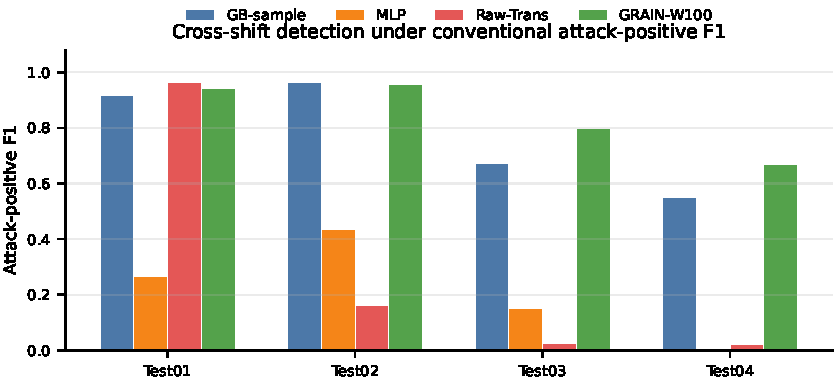
\includegraphics[width=0.98\textwidth]{figures/fig3_main_results.pdf}
\caption{Cross-shift attack-positive F1. Raw-Trans is strong in the known setting but unstable under vehicle and attack shifts, while GRAIN-W100 remains comparatively stable.}
\label{fig:main}
\end{figure}

\subsection{Effect of Feature-Before-Window Representation}
Table~\ref{tab:rawgrain} and Fig.~\ref{fig:rawgrain} isolate the representation effect using W100 rows. Test01 shows that raw-window learning can work when vehicle and attack are known. The shifted settings show the opposite pattern: residual features before aggregation produce a more reliable representation than raw fixed windows.

\begin{table}[t]
\caption{Raw fixed-window pipeline versus \method{} under the same W100 aggregation scale.}
\label{tab:rawgrain}
\centering\small
\begin{tabular}{llcccc}
\toprule
Setting & Pipeline & P & R & F1 & AUPR \\
\midrule
Test01 & GRAIN-W100 & 0.999 & 0.892 & 0.942 & 0.896 \\
Test01 & Raw-Trans & 1.000 & 0.931 & 0.964 & 0.984 \\
Test02 & GRAIN-W100 & 0.984 & 0.931 & 0.956 & 0.935 \\
Test02 & Raw-Trans & 0.087 & 1.000 & 0.160 & 0.049 \\
Test03 & GRAIN-W100 & 1.000 & 0.662 & 0.797 & 0.925 \\
Test03 & Raw-Trans & 1.000 & 0.013 & 0.026 & 0.271 \\
Test04 & GRAIN-W100 & 0.936 & 0.519 & 0.668 & 0.785 \\
Test04 & Raw-Trans & 0.011 & 0.979 & 0.022 & 0.173 \\
\bottomrule
\end{tabular}
\end{table}

\begin{figure}[t]
\centering
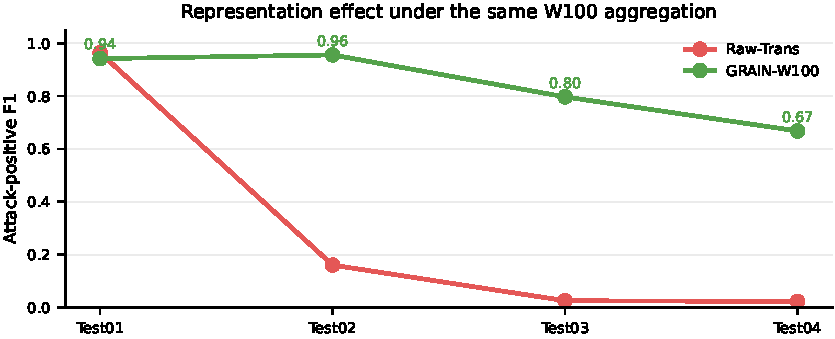
\includegraphics[width=0.92\textwidth]{figures/fig4_raw_vs_grain.pdf}
\caption{Representation comparison at W100. The raw-window Transformer peaks in Test01 but collapses in shifted settings; GRAIN-W100 is less sensitive to the shift.}
\label{fig:rawgrain}
\end{figure}

\subsection{Contribution of Local Behavior Features}
Ablation on Test04 identifies same-ID timing as the strongest local signal in the current implementation. Removing same-ID timing sharply degrades F1, and timing alone outperforms the full safe-feature row. Therefore the present evidence supports a narrower mechanism claim: the main gain comes from making timing disruptions explicit before aggregation. Payload and ID-behavior features remain useful design hooks, but their independent contribution is weak in this setup.

\begin{table}[t]
\caption{Feature-group ablation on CT\&T Test04.}
\label{tab:ablation}
\centering\small
\begin{tabular}{lccccccc}
\toprule
Variant & P & R & F1 & FNR & FPR & AUPR & R@1e-3 \\
\midrule
Timing only & 0.771 & 0.491 & 0.600 & 0.509 & 0.000 & 0.425 & 0.491 \\
Full safe features & 0.740 & 0.354 & 0.479 & 0.646 & 0.000 & 0.255 & 0.355 \\
w/o CAN ID & 0.740 & 0.355 & 0.480 & 0.645 & 0.000 & 0.265 & 0.355 \\
w/o payload stats & 0.740 & 0.354 & 0.479 & 0.646 & 0.000 & 0.255 & 0.355 \\
w/o payload delta & 0.740 & 0.354 & 0.479 & 0.646 & 0.000 & 0.255 & 0.355 \\
w/o same-ID timing & 0.005 & 0.249 & 0.009 & 0.751 & 0.056 & 0.057 & 0.067 \\
\bottomrule
\end{tabular}
\end{table}

\begin{figure}[t]
\centering

\includegraphics[width=0.92\textwidth]{figures/fig5_ablation.pdf}
\caption{Ablation on Test04. Same-ID timing residuals dominate the current implementation; payload and ID groups require further evidence before being claimed as primary contributors.}
\label{fig:ablation}
\end{figure}

\subsection{Sensitivity to Aggregation Window}
W10, W20, and W100 behave differently across settings. Short windows are stronger in Test01 and Test02, while W100 is stronger in Test03 and Test04. This result should be read as sensitivity evidence, not as a test-time hyperparameter search. The main claim is representation-level stability, not a universal best window length.

\subsection{Supplementary Low-False-Alarm Operating Points}
Score-based operating analysis is supplementary. Fig.~\ref{fig:opfpr} compares AUPR and fixed-FPR recall on Test04 for rows with comparable scores. These metrics are useful for deployment discussions, but they should not be mixed with thresholded F1 or compared to prior papers without score outputs.

\begin{figure}[t]
\centering
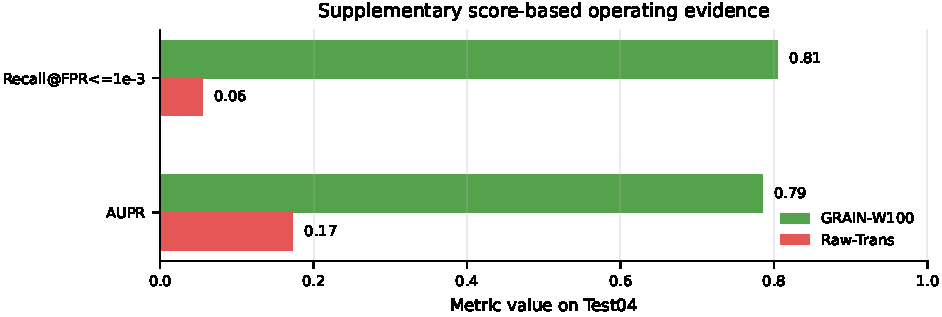
\includegraphics[width=0.92\textwidth]{figures/fig6_operating.pdf}
\caption{Supplementary Test04 operating evidence. AUPR and fixed-FPR recall use score outputs and should be interpreted separately from thresholded F1.}
\label{fig:opfpr}
\end{figure}

\subsection{Diagnostic Rule and Statistical Checks}
Simple single-signal detectors are diagnostic checks only. They test whether \method{} reduces to one threshold over timing or payload change. They are not used as recent state-of-the-art competitors and should remain outside the main comparison.

\section{Discussion}
\subsection{What the Current Evidence Supports}
The strongest current claim is that same-ID residual extraction before window aggregation improves stability over a raw fixed-window Transformer under shifted CT\&T settings. The data do not support an unrestricted multi-feature superiority claim. The ablation indicates that timing residuals are the dominant signal in the present implementation.

\subsection{Failure Modes and Scope}
\method{} is supervised and still needs labelled normal/attack data. It does not recognize unseen attack names. It detects visible local disruptions in timing, payload continuity, or local ID behavior. Attacks that preserve these properties can be missed. The method also reduces but does not remove dependence on vehicle-specific distributions.

\subsection{Comparability to Prior Work}
Prior reported aggregate metrics cannot be directly compared with attack-positive F1 unless the positive class, averaging rule, threshold rule, and confusion matrix are available. For this reason, the paper compares reproduced local rows under a common metric definition and treats score metrics as supplementary. Stronger comparison to recent self-supervised, signal-level, graph, and sequence IDS pipelines requires local reproduction under the same split and metric definitions.

\subsection{Missing Deployment Evidence}
Because \method{} is positioned as a lightweight pipeline, future revisions should report feature-extraction throughput, inference latency per window, model size, CPU-only runtime, and memory usage. Without these measurements, lightweight deployment should be treated as a design motivation rather than a proven result.

\section{Conclusion}
\method{} demonstrates that same-ID local behavior residuals before window aggregation are a useful lightweight representation for cross-shift CAN IDS. The current evidence is strongest for timing residuals: they make local disruptions visible before the window classifier receives the sample and improve shifted-setting stability compared with a raw fixed-window baseline. The method remains supervised and limited to attacks that produce visible timing, payload, or local ID-behavior disruptions. Future work should combine this residual representation with self-supervised training, decoded signal features, graph context, online adaptation, and real-time deployment evaluation.

\begin{thebibliography}{18}
\bibitem{alkhatib2022} Alkhatib, N., Mushtaq, M., Ghauch, H., Danger, J.L.: CAN-BERT do it? Controller area network intrusion detection system based on BERT language model. arXiv:2210.09439 (2022)
\bibitem{blevins2021} Blevins, D.H., Moriano, P., Bridges, R.A., Verma, M.E., Iannacone, M.D., Hollifield, S.C.: Time-based CAN intrusion detection benchmark. arXiv:2101.05781 (2021)
\bibitem{canet2019} Hanselmann, M., Strauss, T., Dormann, K., Ulmer, H.: CANet: An unsupervised intrusion detection system for high dimensional CAN bus data. arXiv:1906.02492 (2019)
\bibitem{checkoway2011} Checkoway, S., McCoy, D., Kantor, B., Anderson, D., Shacham, H., Savage, S., Koscher, K., Czeskis, A., Roesner, F., Kohno, T.: Comprehensive experimental analyses of automotive attack surfaces. In: USENIX Security Symposium (2011)
\bibitem{cho2016} Cho, K.T., Shin, K.G.: Fingerprinting electronic control units for vehicle intrusion detection. In: USENIX Security Symposium, pp. 911--927 (2016)
\bibitem{cho2017} Cho, K.T., Shin, K.G.: Viden: Attacker identification on in-vehicle networks. In: ACM CCS, pp. 1109--1123 (2017)
\bibitem{koscher2010} Koscher, K., Czeskis, A., Roesner, F., Patel, S., Kohno, T., Checkoway, S., et al.: Experimental security analysis of a modern automobile. In: IEEE Symposium on Security and Privacy, pp. 447--462 (2010)
\bibitem{lampe2024} Lampe, B., Meng, W.: can-train-and-test: A curated CAN dataset for automotive intrusion detection. Computers \& Security 140, 103777 (2024)
\bibitem{liu2026} Liu, Q., Song, R., Cui, L., Zhang, H., Sun, Y., Sun, L.: MIDS: Detecting stealthy masquerade and tampering attacks on CAN bus via bidirectional Mamba. arXiv:2606.18599 (2026)
\bibitem{miller2015} Miller, C., Valasek, C.: Remote exploitation of an unaltered passenger vehicle. Black Hat USA (2015)
\bibitem{shahriar2022} Shahriar, M.H., Xiao, Y., Moriano, P., Lou, W., Hou, Y.T.: CANShield: Deep learning-based intrusion detection framework for controller area networks at the signal-level. arXiv:2205.01306 (2022)
\bibitem{song2016} Song, H.M., Kim, H.R., Kim, H.K.: Intrusion detection system based on the analysis of time intervals of CAN messages for in-vehicle network. In: ICOIN, pp. 63--68 (2016)
\bibitem{taylor2015} Taylor, A., Leblanc, S., Japkowicz, N.: Frequency-based anomaly detection for the automotive CAN bus. In: World Congress on Industrial Control Systems Security, pp. 45--49 (2015)
\bibitem{verma2020} Verma, M.E., Bridges, R.A., Hollifield, S.C., Iannacone, M.D., Moriano, P.: ROAD: The real ORNL automotive dynamometer controller area network intrusion detection dataset. arXiv:2012.14600 (2020)
\bibitem{wang2023} Wang, K., Jiang, Q., Wang, B., Zhang, Y., Wu, Y.: Effective in-vehicle intrusion detection via multi-view statistical graph learning on CAN messages. arXiv:2311.07056 (2023)
\bibitem{xcanids2023} Jeong, S., Lee, S., Lee, H., Kim, H.K.: X-CANIDS: Signal-aware explainable intrusion detection system for controller area network-based in-vehicle network. arXiv:2303.12278 (2023)
\end{thebibliography}
\end{document}
